\documentclass[a4paper, 11pt, oneside]{article}

\usepackage[utf8]{inputenc}
\usepackage[T1]{fontenc}
\usepackage[english]{babel}
\usepackage{fullpage}
\usepackage{enumerate}
\usepackage{enumitem}
\usepackage{graphicx}
\usepackage{url}
\usepackage{float}
\usepackage{titling}
\renewcommand\maketitlehooka{\null\mbox{}\vfill}
\renewcommand\maketitlehookd{\vfill\null}

\newcommand{\ClassName}{INFO-0045: Introduction to Computer Security}
\newcommand{\ProjectName}{Project 1 - Firewalls\\Part 1 - Drawing of the Network}
\newcommand{\AcademicYear}{2021 - 2022}

%%%% First page settings %%%%

\title{\ClassName\\\vspace*{0.8cm}\ProjectName\vspace{1cm}}
\author{Maxime Goffart \\180521 \and Olivier Joris\\182113}
\date{\vspace{1cm}Academic year \AcademicYear}

\begin{document}

%%% First page %%%

\begin{titlingpage}
{\let\newpage\relax\maketitle}
\end{titlingpage}

\newpage

%%%%%%%%%%%%%%%%%%%%%%%%%%%%%%%%%%%%%%%%%%

\section{Drawing of the network}
\paragraph{}We can represent the described network by the following diagram:

\begin{figure}[H]
  \makebox[\textwidth][c]{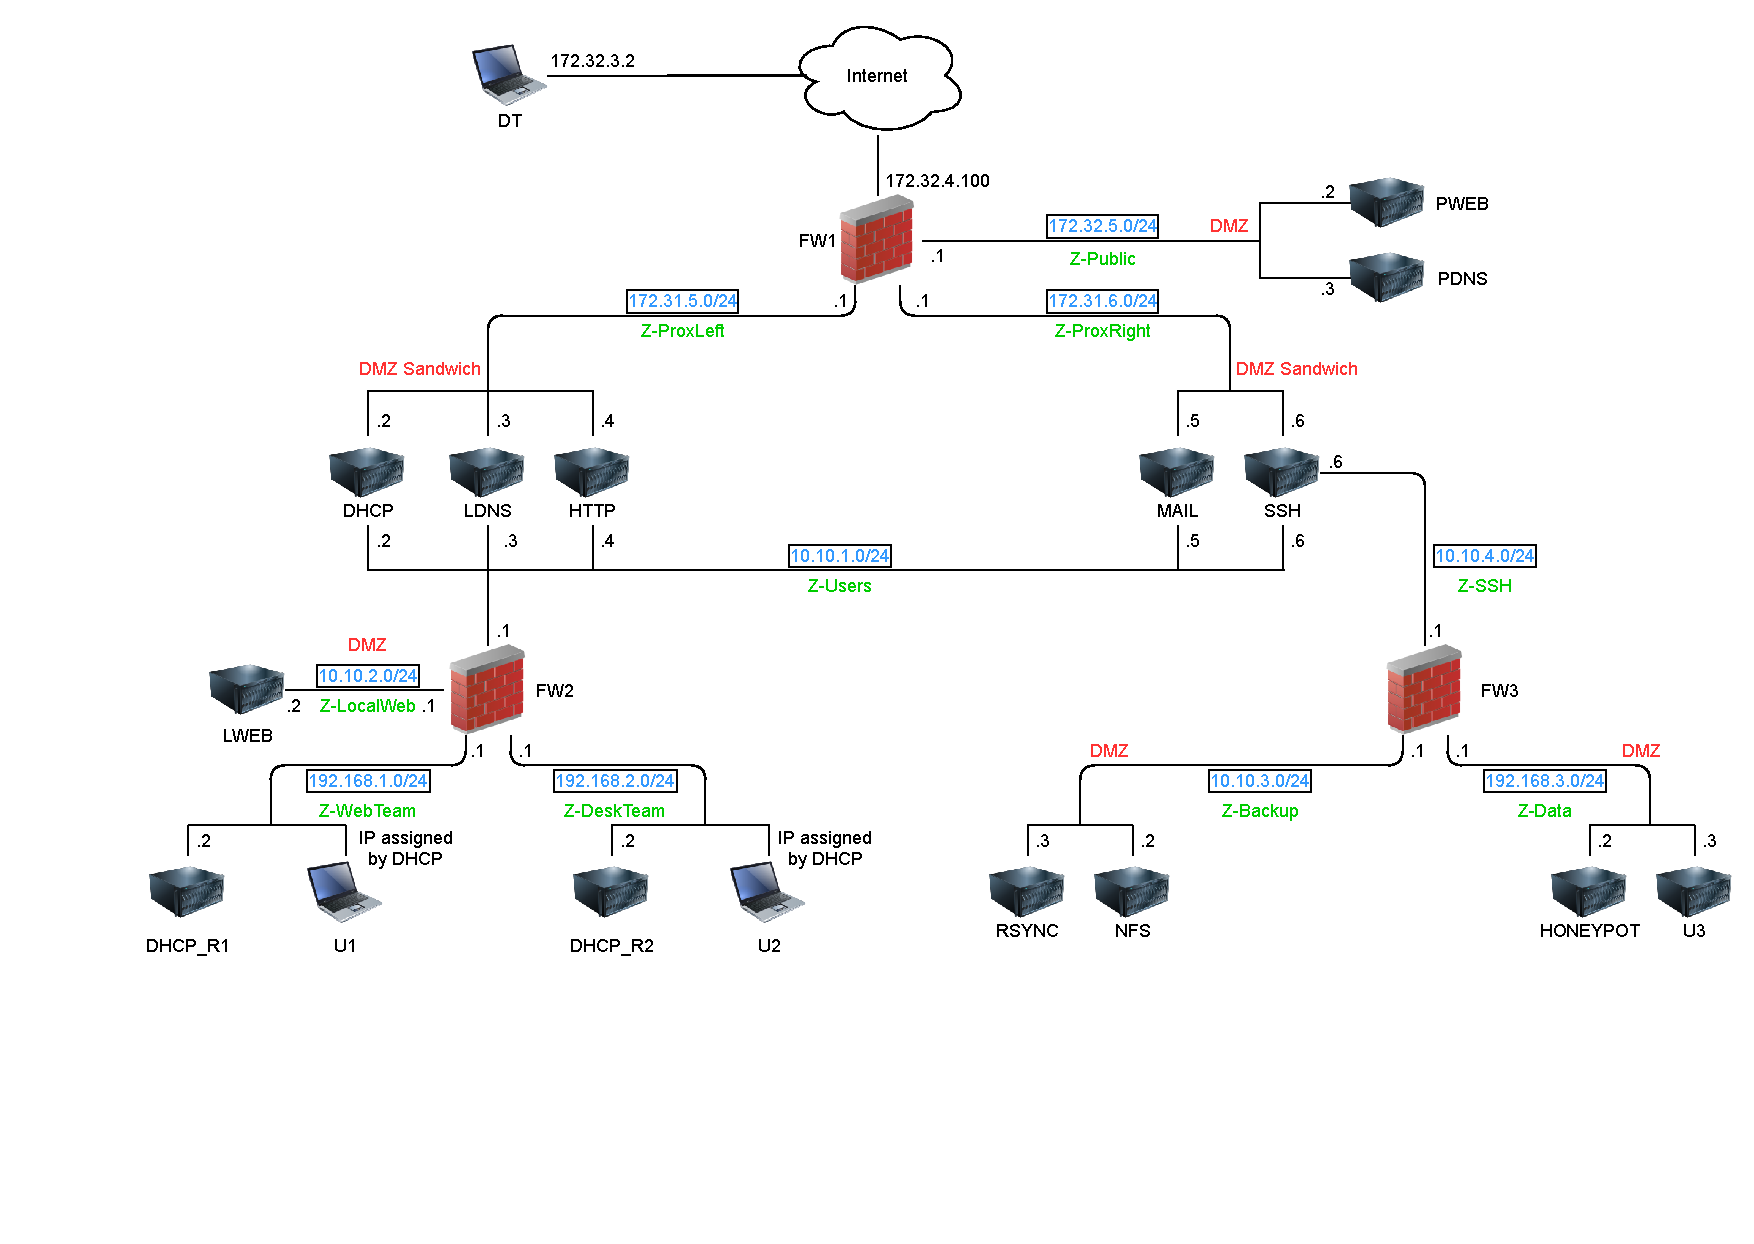
\includegraphics[width=1.2\textwidth]{../drawing/network.pdf}}%
  \caption{Network topology}
  \label{fig:key}
\end{figure}

\section{Zones and their order per firewall}

\subsection{Zones}
\paragraph{}We have the following zones:

\begin{itemize}
\item \texttt{Z-Public} is the zone associated to devices that can be reach from the Internet. It corresponds to the subnet 172.32.5.0/24.
\item \texttt{Z-ProxLeft} is the zone associated to the DHCP, LDNS, and HTTP(S) services. It corresponds to the subnet 172.31.5.0/24.
\item \texttt{Z-ProxRight} is the zone associated to the mail (IMAP and SMTP) and SSH services. It corresponds to the subnet 172.31.6.0/24.
\item \texttt{Z-Users} is the zone associated to the users of the network. It corresponds to the subnet 10.10.1.0/24.
\item \texttt{Z-LocalWeb} is the zone associated to the local web server. It corresponds to the subnet 10.10.2.0/24.
\item \texttt{Z-WebTeam} is the zone associated to the web team. It corresponds to the subnet 192.168.1.0/24.
\item \texttt{Z-DeskTeam} is the zone associated to the desk team. It corresponds to the subnet 192.168.2.0/24.
\item \texttt{Z-SSH} is the zone associated to the SSH relay. It corresponds to the subnet 10.10.4.0/24.
\item \texttt{Z-Backup} is the zone associated to the backup servers. It corresponds to the subnet 10.10.3.0/24.
\item \texttt{Z-Data} is the zone associated to the data servers. It corresponds to the subnet 192.168.3.0/24.
\end{itemize}

\subsection{Order of zones per firewall}
\paragraph{}For firewall \texttt{FW1}, we have the following order of zones based on decreasing security level:
\begin{enumerate}[label={\arabic*)}]
\item \texttt{Z-ProxLeft} because these services should not be reachable from outside except for the replies of HTTP(S) and DNS protocols.
\item \texttt{Z-ProxRight} because the mail server and ssh relay should receive connections from outside.
\item \texttt{Z-Public} because the servers inside this zone are intended for public use.
\end{enumerate}

\paragraph{}For firewall \texttt{FW2}, we have the following order of zones based on decreasing security level:
\begin{enumerate}[label={\arabic*)}]
\item \texttt{Z-DeskTeam} because it should have the highest level of security.
\item \texttt{Z-WebTeam} because it should have the same restrictions as \texttt{Z-DeskTeam}. Yet, it also need access to the RSYNC server to backup web data and they need access to the FTP server of LWEB to modify web pages.
\item \texttt{Z-LocalWeb} because it should be accessible only by people from \texttt{Z-WebTeam} and \texttt{Z-DeskTeam}.
\item \texttt{Z-Users} because it should be accessible by anyone from \texttt{Z-WebTeam} and \texttt{Z-DeskTeam} because they need to access the proxies, the mail server, and the SSH relay.
\end{enumerate}

\paragraph{}For firewall \texttt{FW3}, we have the following order of zones based on decreasing security level:
\begin{enumerate}[label={\arabic*)}]
\item \texttt{Z-Backup} because it is highly sensible. We definitely do not want anyone without proper permissions to access the servers inside it.
\item \texttt{Z-Data} because it should be accessible only by a few people or a few servers.
\item \texttt{Z-SSH} because it is under less restrictions than the previous zones.
\end{enumerate}

%%%%%%%%%%%%%%%%%%%%%%%%%%%%%%%%%%%%%%%%%%

\end{document}